% !TeX program = pdflatex

\documentclass[11pt, conference]{IEEEtran}
\usepackage{hyperref}
\hypersetup{unicode, bookmarksnumbered, bookmarksopen, breaklinks, hidelinks, pdfstartview=FitH}
\AtBeginDocument{\urlstyle{tt}}
\usepackage{amsmath, amsfonts, amssymb}
\usepackage{txfonts}
\usepackage{graphicx, xcolor}
\graphicspath{{figures/}}
\usepackage{cite}
\usepackage{booktabs}
%\usepackage{subcaption}
\usepackage{float}
\newcommand{\tcr}{\textcolor{red}}

\let\Mean\overline
\def\D{\mathrm{d}}
\def\Email#1{\href{mailto:#1@shanghaitech.edu.cn}{#1}}

\begin{document}

\title{Athernet: A Toy Network}
\author{%
\IEEEauthorblockN{Yifan Cao \qquad Weitian Wang}
\IEEEauthorblockA{ShanghaiTech University \\
\texttt{\char`\{\Email{caoyf}, \Email{wangwt}\char`\}@shanghaitech.edu.cn}}
}
\maketitle

\section{Introduction}

As the project for CS120, We implement Athernet, a toy net that uses acoustic signal or sound to transmit information through the 
audio connection. We implemented the physical layer and MAC layer of the network. We also implemented a NAT for
Athernet to make it communicate with internet and an FTP client for Athernet nodes on UDP protocol so we can download files 
for the off-net Athernet node via the audio connection. In this project, we use C++ for Athernet implementation and use python to
implement part of NAT for Internet transmission.

\section{Project 1: Acoustic Connection}

In this project, we work on physical layer of Athernet. we choose ASIO, a computer sound card driver protocol for digital audio that provides a low-latency and high fidelity
interface between a software application and a computer's sound card to generate and receive sound wave, and develop our project based 
on JUCE, a C++ application framework which provides powerful support for audio transmission. We encode the transfering bitstream as samples 
of sound wave by PSK method, packed with header wave as a physical layer frame. As a result, we successfully transmit 10000 bits by our own microphone and speaker in 15 seconds
with acuuracy of 100 percent. However, the transmission is fragile and susceptible to noise from surrouding.

\subsection{Modulation}

We choose PSK to modulate bitstream. In original design (without OFDM), we use the wave $1 \times cos(2\pi \times 5000 x + \pi)$ to represent 1, and
$  1 \times cos(2\pi \times 5000 x) = -cos(2\pi \times 5000 x)$ to represent 0. We choose the sample rate of 48000Hz, and by fully test the harwares, 
we find that 400 bits per frame and 48 samples per bit best fit our devices, giving consideration of both accuracy and bandwidth.

As for header wave, it is also a sin wave that start with frequency 200Hz, and continuously increases its frequency until 10000Hz, and after that, its
frequency decreses at the same speed to 2000Hz, which is shown in Fig.1

\begin{figure}[!h]
	\centering
	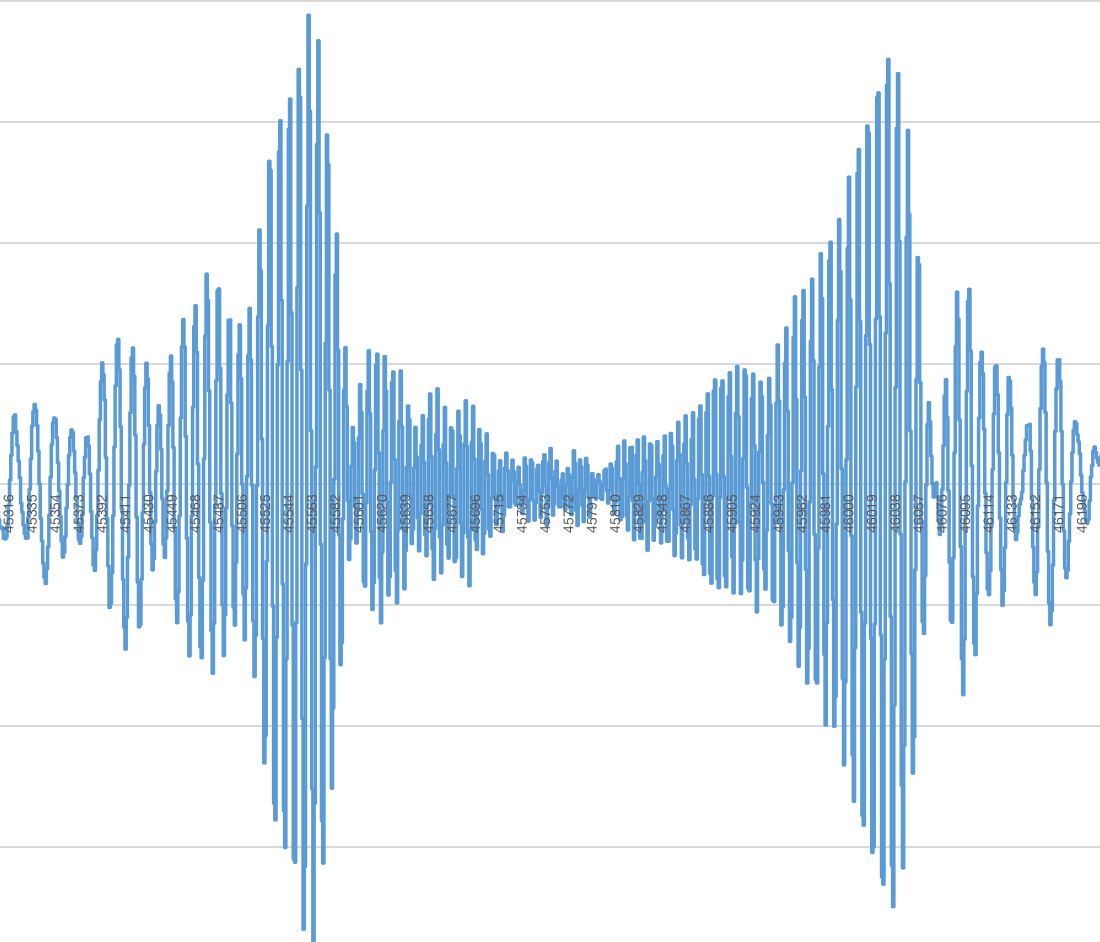
\includegraphics[scale=0.4]{header_wave.png}
	\caption{header wave}\label{}
	\end{figure}

\subsection{\tcr{Demodulation}}

We use an algorithm to demodulate the audio samples to bits. There are two states: synchronizing and decoding.

\subsubsection{Synchronization}

In the synchronizing state, the program is reading the samples and finds if a header arrives. If it ensures that it hears a header, it switches to the decoding state with the accurate start of this frame recorded.

When synchronizing, we are looking at a number of samples, which is as many as that of a header. We expect to decide how much could these samples fit the header. A variable \textsf{syncPower} is used to estimate the goodness of fit. Given header $H$ and samples $S$ with length $N$, this value is defined as
\[
\textsf{syncPower} = \sum_{i=1}^N H_i \cdot S_i.
\]
The larger \textsf{syncPower} is, the better the samples fit the header. We set a threshold value that \textsf{syncPower} must exceed if the samples are considered as a header. We use a variable called \textsf{maxSyncPower} which records the maximum \textsf{syncPower} value that exceeds the threshold in the near past. If \textsf{maxSyncPower} has not been changed for a period of time, and the current value of it does exceed the threshold, we conclude that the time \textsf{maxSyncPower} appears is exactly the accurate start of the packet. Here we need to wait for a period of time, in case the best fit is used.

To be stricter, we apply an additional strategy to the synchronization algorithm. When we arrive at the header at some time, the \textsf{syncPower} should be obviously large than that of even 1 sample deviation. Taking advantage of this feature, we allow the update of \textsf{maxSyncPower} only if the \textsf{syncPower} exceeds a fixed multiple of \textsf{power}, which roughly estimates the power of the recent samples. Initially it is $0$, and it is updated according to the equation
\[
\textsf{power}_i = \frac{63}{64} \cdot \textsf{power}_{i-1} + \frac{S_i^2}{64},
\]
where $i$ is the sample number and $S_i$ is the sample value. In this equation, the most recent sample $S_i$ is merged into \textsf{power} with ratio $1/64$, while the previous \textsf{power} is reduced to $63/64$ of the original, since it represents some older values.

\subsubsection{Decoding}

In the decoding state, the program has already found the start of this frame. If a bit is represented by $s$ samples, and this frame includes $n$ bits, the number of samples we should receive after the header is $n \cdot s$. We split the samples into groups of length $s$, where each group contains samples that represent a common bit. These samples should roughly have the form
\[
s(t) =
\begin{cases}
A\sin(2\pi f_ct), & \text{binary 1}, \\
A\sin(2\pi f_ct + \pi), & \text{binary 0},
\end{cases}
\]
which is similar to those the sender generates. To decode the samples, multiply their values with $A\sin(2\pi f_ct)$. The form then becomes
\[
s(t) =
\begin{cases}
A\sin^2(2\pi f_ct), & \text{binary 1}, \\
-A\sin^2(2\pi f_ct), & \text{binary 0}.
\end{cases}
\]
In other words, if the bit is $1$, the values should chiefly be positive, otherwise negative. We sum these values up, and conclude the bit is $1$ if the sum is positive, and $0$ otherwise.

\subsection{Higher bandwidth: OFDM}

OFDM is a method to encode bits on multiple carrier frequencies. 'O' is orthogonal, and if we use two or more sin waves to transmit simultaneously,
the superimposed wave is able to carry information from all channels, as long as they are orthogonal. A simplest orthogonal case is $cos(x)$ and $cos(2x)$,
and we can modulate two channels information in the form of 
\[
    A(\text{bit}_1 \times 2 - 1)cos(fx) + B(\text{bit}_2 \times 2 - 1)cos(2fx)\\
\]
and in this case we can trnasmit 2 bits at once. In other words, the bandwidth doubles.

In demodulate stage, we multiply the received waves with two carrier waves, and therefore decode two coreespoding bits.
In practice, we adopt a more reliable approach for the case of two frequencies. Firstly, 4 carrier waves are generated at the
very beginning, they are:
\[
    \begin{cases}
    A(\text{bit}_1 \times 2 - 1)cos(fx+\pi) + B(\text{bit}_2 \times 2 - 1)cos(2fx + \pi) \dots 0 \\
    A(\text{bit}_1 \times 2 - 1)cos(fx+\pi) + B(\text{bit}_2 \times 2 - 1)cos(2fx) \dots 1\\
    A(\text{bit}_1 \times 2 - 1)cos(fx) + B(\text{bit}_2 \times 2 - 1)cos(2fx + \pi) \dots 2\\
    A(\text{bit}_1 \times 2 - 1)cos(fx) + B(\text{bit}_2 \times 2 - 1)cos(2fx) \dots 3\\
    \end{cases}
\]
and each of them is corresponding to a digit of 0,1,2,3. Then, we multiply each carrier wave with received wave respectively, track the carrier wave with the largest product, and decode the two
bits as the corresponding digits of the waves.
\section{Project 2: Multiple Access}

In project two, our hardware devices change from commercial speakers and microphones to sound cards and calbles, which allows us to transmit in baseband and use a few samples to 
encode a bit (we choose 3 samples per bit), and we mainly work on MAC layer of Athernet. We redesign the frame header, adding src\_addr, dst\_addr, sequence number, type, length fields,
as well as a CRC checksum. For Athernet nodes, we establish a state-machine for each node, using multithreding to archive transmitting and receiving at same time, and also ACK and retrasmission
mechanism. We also design amd support MacPing and MacPerf command to test the latency and bandwith of Athernet. Finally, to avoid conflict, we implement CSMA to detect the channel and backoff when transmission detected.

\subsection{The Packet Structure}

In the packet, we reserve some bits to store necessary fields.
\begin{itemize}
\item The first 8 bits are type filed, i.e. they type of this packet, such as data frame, MacPing(request, reply), MacPerf, ACK...
\item The second 8 bits are sequence number field, which is essential for ACK and retrasmission.
\item The thrid 8 bits are dst\_addr field. 
\item The fourth 8 bits are src\_addr field.
\item The fifth 8 bits are length filed, which tells the length of the frame's data.
\end{itemize}

\subsection{ACK and retrasmission}

ACK and retransmission are fundamental to archive a reliable transmission. Due to the fragileness of hardware trasmission, packets in 
Athernet suffer from a series of failure, like lost in cable and reversal for bits. Take data packets for example, when Athernet nodes receive
a data packet with sequence number $K$ and its CRC checkusm is 'good', the receiver node will reply an ACK packet with sequence number $K$, and when the
trasmitting node receive the ACK of this packet, the transmission of packet $K$ is treated as successfully, else retransmission is needed. Trasmission occurs
in four situations,
\begin {itemize}
\item The data packet is lost, i.e. the receiver does not receive packet $K$.
\item some bits are changed during the transmission, i.e. the CRC check does not pass.
\item The ACK packet is lost.
\item Both data packet and ACK packet are transmitted correctly, but timeout occurs.
\end {itemize}
In transmitting node, we either maintain a thread pool that keeps the duration of all current transmitting packets using std::condition\_variable.wait\_until method
in C++, or just iteratively check the duration in sending thread. When timeout occurs, the transmitting thread abort the previous transmission and retransmit the abrted packet.

For data transmission in project 2, we found that stop-and-wait strategy does not meet the requirement in performance, so for the relatively small data file, we just transmit all
packets at beginnning, and after receiving ACK packets, it continuouly transmit the rest packets without ACK replies, until all packets are successfully transmitted.

\subsection{CRC}
To ensure the correctness of transmission, we introduce CRC check. We choose CRC8 with CRC polynomials
\[
    x^8 + x^2 + x + 1 \dots 0\text{x}07
\]
We compute the CRC checksum when constructing data packets, appending the result in the end of packets, and in receiver node, we recompute the CRC checksum with same algorithm and compare with the appended one to do the corectness check.
\subsection{The \textsf{macperf} Utility}
We implementation perf packet in MAC layer, which is a utility to measure the throughput of Athernet. We design the MACperf packet with almost same header as data packet(no length field), and tramit 1000 random bits as 
payload for each MACperf packet. The MACperf controller sends packets with best effort, while counting the ACK received for each second, and print the measured throughput on the screen.

\subsection{The \textsf{macping} Utility}

We also implement ping packet in MAC layer to measure the latency. The MacPing packets' header is same as MacPerf packets, but the random payload is only a byte long.

When node1 tries to do the MacPing meausrement to node2, it sends one MacPing request packet per second, and begin a timer when the request packet is delivered to physical layer. For node2, the MacPing request packet is replied
as soon as possible with a MacPing reply packet, and when node1 receive the MacPing reply packet, it stops the corresponding timer, printing the duration which is just the RTT of the packet.

Note that in both MacPerf and MacPing packets, adrress is taken into consideration and need to be handled carefully.

\subsection{\tcr{CSMA}}

Since it is possible that the channel (i.e. audio cable) is used by someone else, sending a packet may fail. To avoid this, we listen to the channel before we send a packet. The protocol is as follows.
\begin{itemize}
\item Initialize the safe bit to false.
\item At a given time, the packet detection thread reads the \textsf{power} value. If it exceeds a threshold value, someone else is using this channel, and set the safe bit to false. Otherwise, set it to true.
\item When a thread wants to send a packet (a normal one or an ACK), it checks the safe bit. If it is false, wait (\emph{back off}) for a few milliseconds and check the safe bit again, until this bit is true and then it may send a packet since the channel is considered free.
\end{itemize}

\section{Project 3: NAT}

In project three, we build a gateway for the Athernet and in this way, Athernet devices is able to communicate with Internet. With NAT, we successfully transmit data by UDP packet between Athernet nodes and Internet. 
We further support ICMP protocol packets so that Athernet devices can ping Internet devices, and vice versa. In our project, the ping latency is about 140ms.

\subsection{\tcr{Forwarding packets between Athernet and Internet}}

We use different languages to establish connections in the Athernet and Internet. For the gateway, we need to share data between the two connections, so we use temporary files on the disk. To send a packet from Athernet to Internet, the working flow is as follows.
\begin{itemize}
\item $A$ sends a packet to $B$ via the Athernet.
\item The Athernet connection of $B$ stores the packet to a file $F$, and creates a notification file \textsf{ATH\_NOTIFY} in the current directory.
\item The Internet connection of $B$ has a thread waiting for the notification file from the Athernet, \textsf{ATH\_NOTIFY}. As soon as it finds this file in the current directory, it deletes it, changes the source of this packet to $B$, and sends the packet in $F$ to the destination (i.e. $C$), which is also specified in the packet.
\end{itemize}

To send a packet from Internet to Athernet, the working flow is as follows.
\begin{itemize}
\item $C$ sends a packet to $B$ via the Internet.
\item The Athernet connection of $B$ stores the packet to a file $F'$, and creates a notification file \textsf{INT\_NOTIFY} in the current directory.
\item The Athernet connection of $B$ has a thread waiting for the notification file from the Internet, \textsf{INT\_NOTIFY}. As soon as it finds this file in the current directory, it deletes it and sends the packet in $F'$ to the destination (i.e. $A$), which is also specified in the packet.
\end{itemize}

\subsection{ICMP ping}
An important feature of Athernet is it support ICMP ping between Athernet and Internet. We implement both ping from Athernet devices to Internet devices and vice versa (ping from external devices). The working flow of
ping from Athernet devices is (here we specify node1 is the Athernet node, node2 is the NAT node, and node3 is an internet device):
\begin{itemize}
    \item node1 translates node3's IP address into bits, creates ICMP request packet, and starts a timer.
    \item node1 delivere the packet to physical layer and transmit it to node2.
    \item node2 check the packet's TYPE field, and if it is a ICMP ping request, node2 translate the IP address and write it to a notifying file.
    \item node2's python process detects the file, reads the IP address and sends a Internet ICMP ping request packet to node3.
    \item node3 automaticly reply with ICMP ping reply packet.
    \item node2's python process receive the reply, and notify C++ process to continue.
    \item node2 creates and sends an ICMP ping reply packet to node1.
    \item node1 receives the packet and counts the duration.
\end{itemize}
The working flow of ping from external is basically similar, but we need more operations like:
\begin{itemize}
    \item we ban the system ICMP reply by modifying the Windows firewall.
    \item we use scapy library to catch ICMP packets and store the IP payload of the ping request.
    \item Athernet nodes should be able to reply ICMP request as soon as possible.
    \item to reply the Internet ICMP request, we need to modify the TYPE filed of ICMP header, and recalculate the ICMP checksum.
\end{itemize}


\section{\tcr{Project 4: FTP}}

In this project, we implement an Athernet client of the \emph{file transfer protocol} (FTP), so that the user may retrieve files from the Internet. This depends on the gateway implemented in the last project.

The Athernet client node may specify the address of the FTP server, and is able to use FTP control commands. Among these commands, some simply sends short messages and receives short responses, such as \textsf{USER}, \textsf{PASS}, \textsf{PWD}, \textsf{CWD}, \textsf{PASV}. Some can initiate data transmission, such as \textsf{LIST}, \textsf{RETR}. In order to simplify the behavior, at the client side, \textsf{LIST} prints the data to \textsf{stdout}, and \textsf{RETR} saves the data as a file in the current directory.

Assume that there are three nodes: $A$ (Athernet), $B$ (gateway), and $C$ (Internet). The working flow is as follows.
\begin{itemize}
\item $A$ specifies the address of the FTP server and tells $B$.
\item $B$ establishes an Internet connection with $C$. If success, there may be a response from $C$.
\item $B$ tells $A$ the connection result and optionally with the responses from $C$.
\item $A$ prints a message saying if the connection is established or not, optionally with the response.
\item $A$ sends the FTP control command to $B$.
\item $B$ forwards the command to $C$.
\item $C$ sends the response to $B$, optionally with data if the command is \textsf{LIST} or \textsf{RETR}.
\item $B$ forwards the response to $A$, optionally with data.
\item $A$ receives the response, optionally with data. If the command sent is \textsf{LIST}, print it out; if it is \textsf{RETR}, save to a file. Then it prints the response.
\end{itemize}
Note: All the packets in Athernet are sent under a stop-and-wait protocol. The next packet may be sent only if the ACK of the current packet is received.

\clearpage

\begin{thebibliography}{1}
\bibitem{stan} Stanford University EE102B. \emph{Analog Transmission of Digital Data: ASK, FSK, PSK, QAM}. \url{https://web.stanford.edu/class/ee102b/contents/DigitalModulation.pdf}.
\bibitem{stack} Stack Overflow. \emph{Translate CRC8 from C to Java}. \url{https://stackoverflow.com/questions/25284556/translate-crc8-from-c-to-java}.
\bibitem{pysoc} Python 3.7.2 Documentation. \emph{\textsf{socket} --- Low-level networking interface}. \url{https://docs.python.org/3/library/socket.html}.
\bibitem{ping} GitHub Gist. \emph{A pure python ping implementation using raw socket}. \url{https://gist.github.com/pklaus/856268}.
\end{thebibliography}

\end{document}
